\documentclass[12pt, letterpaper, oneside]{article}
\usepackage{amsmath}
\usepackage{amssymb}
\usepackage{csquotes}
\usepackage{float}
\usepackage{hyperref}
\usepackage{tikz}
\usetikzlibrary{arrows, automata, positioning, shapes.geometric}
\usepackage{parskip}
\usepackage{xcolor}

\hypersetup{
  colorlinks=true,
  linkcolor=blue,
  filecolor=magenta,
  urlcolor=blue,
}

\begin{document}

% =============================================================================
\section{What exactly is an irrational number?}
% =============================================================================

What exactly is an irrational number? An irrational number is a real number that cannot be expressed as a fraction
of two integers. In other words, it cannot be written in the form \(\frac{p}{q}\), where \(p\) and \(q\) are integers
and \(q \neq 0\).

But in the description above, we mentioned that irrational numbers are real numbers. But is there a way to define an
irrational number without using the concept of real numbers? Yes, we can define irrational numbers using the concept of
decimal expansions. An irrational number is a number that has a non-terminating and non-repeating decimal expansion.
This means that when you write the number in decimal form, the digits go on forever without ever settling into a
repeating pattern. For example, the number \(\pi\) (approximately 3.14159...) is irrational because its decimal
expansion goes on forever without repeating. Similarly, the square root of 2 (approximately 1.41421...) is also
irrational for the same reason.

But how can we prove that an irrational number cannot be expressed as a fraction of two integers? One common method is
to use a proof by contradiction. For example, let's prove that \(\sqrt{2}\) is irrational. Suppose that \(\sqrt{2}\) is
rational, meaning it can be expressed as a fraction \(\frac{p}{q}\), where \(p\) and \(q\) are integers with no common
factors (i.e., the fraction is in its simplest form). Then we have:
\[\sqrt{2} = \frac{p}{q}\]

Squaring both sides gives:
\[2 = \frac{p^2}{q^2}\]

Multiplying both sides by \(q^2\) gives:
\[2q^2 = p^2\]

This implies that \(p^2\) is even (since it is equal to \(2q^2\)), which means that \(p\) must also be even (because
the square of an odd number is odd). Therefore, we can write \(p\) as \(2k\) for some integer \(k\). Substituting this
back into the equation gives:
\[2q^2 = (2k)^2\]
\[2q^2 = 4k^2\]

Dividing both sides by 2 gives:
\[q^2 = 2k^2\]

This implies that \(q^2\) is also even, which means that \(q\) must be even as well. However, this contradicts our
initial assumption that \(p\) and \(q\) have no common factors (since both are even, they share a factor of 2).
Therefore, our assumption that \(\sqrt{2}\) is rational must be false, and thus \(\sqrt{2}\) is irrational.

Then how can we prove that irrational numbers have non-terminating and non-repeating decimal expansions? We can prove
this by contradiction as well. Suppose that an irrational number has a terminating or repeating decimal expansion. If
it has a terminating decimal expansion, it can be expressed as a fraction of two integers (since any terminating decimal
can be converted to a fraction). If it has a repeating decimal expansion, it can also be expressed as a fraction of two
integers (using the method of converting repeating decimals to fractions). In both cases, this contradicts the
definition of an irrational number. Therefore, irrational numbers must have non-terminating and non-repeating decimal
expansions.

A more formal proof of this can be given using the concept of limits and infinite series. Consider an irrational number
\(x\) with a decimal expansion:
\[x = d_0.d_1d_2d_3\ldots\]

where \(d_0\) is the integer part and \(d_1, d_2, d_3, \ldots\) are the digits after the decimal point. We can express
this decimal expansion as an infinite series:
\[x = d_0 + \frac{d_1}{10} + \frac{d_2}{10^2} + \frac{d_3}{10^3} + \ldots\]

If \(x\) were rational, then this series would either terminate or repeat. However, since \(x\) is irrational, the
series does not terminate or repeat. This means that for any finite number of terms in the series, we can always find
more terms that differ from the previous ones, ensuring that the decimal expansion is non-terminating and non-repeating.

However, there is a very simple explanation of why irrational numbers have non-terminating and non-repeating: they are
\textbf{defined} that way. We human beings created the concept of irrational numbers to describe numbers that cannot be
expressed as fractions of integers. By definition, irrational numbers are those that do not fit into the category of
rational numbers, which are defined as numbers that can be expressed as fractions of integers. Therefore, it is inherent
in the definition of irrational numbers that they have non-terminating and non-repeating decimal expansions.

% =============================================================================
\section{Why do real numbers only consist of rational and irrational numbers?}
% =============================================================================

Simple: \textbf{By definition}. Real numbers are defined as the set of all rational and irrational numbers. This
definition is based on the need to create a comprehensive number system that can represent all possible quantities along
a continuous number line. Rational numbers are those that can be expressed as fractions of integers, while irrational
numbers are those that cannot be expressed as fractions of integers. By combining these two sets of numbers, we obtain
the set of real numbers, which includes all possible values that can be represented on the number line.

When we consider the questions like ``Why irrational numbers are non-terminating and non-repeating?'' or ``Why real
numbers only consist of rational and irrational numbers?'', we must be aware that these concepts are defined by humans.
Because we define them that way, then they have the properties that the definitions specify.

In contrast, suppose one day an extraterrestrial object hits the Earth and the human scientists start to study it. They
find that this object contains two chemical elements that are unknown to us before. Now, can they say that this object
only has these two unknown elements? Could there be more? Yes, there could be more, because the fact that only two
elements are found is just based on our current knowledge and technology. There might be other elements that we have not
yet discovered or identified. In other words, when we face an objective object, we must prove that there are no other
possibilities before we can conclude that only the known possibilities exist.

However, when we talk about mathematical concepts like real numbers, rational numbers, and irrational numbers, we are
dealing with definitions and abstractions created by humans. In this case, we define real numbers as the set of all
rational and irrational numbers. Since this is a definition, there are no other possibilities to consider. The set of
real numbers is \textbf{by definition} the union of rational and irrational numbers, and there are no other types of
numbers included in this definition. Therefore, we don't need to prove that real numbers only consist of rational and
irrational numbers; it is simply a matter of how we have defined these concepts in mathematics. Likewise, we don't need
to prove that irrational numbers have non-terminating and non-repeating decimal expansions; it is also a matter of
definition.

% =============================================================================
\section{Prove: 0.999\ldots = 1}
% =============================================================================

This is an example to show that we can't always trust our intuition in mathematics when it comes to infinite processes
because our daily experiences are based on finite observations.

By intuition, one might think that \(0.999\ldots\) is just a number that is very close to 1, but not equal to it.
However, mathematically, we can prove that \(0.999\ldots\) is indeed equal to 1. And we can prove this in several ways.

The \textbf{first method} involves using fractions. We know that:
\[\frac{1}{3} = 0.333\ldots\]

If we multiply both sides of this equation by 3, we get:
\[3 \times \frac{1}{3} = 3 \times 0.333\ldots\]

This simplifies to:
\[1 = 0.999\ldots\]

Thus, \(0.999\ldots = 1\).

The \textbf{second method} is to use algebra. Let's denote \(x = 0.999\ldots\).

Then, multiplying both sides by 10 gives:
\[10x = 9.999\ldots\]

Now, subtract the original equation from this new equation:
\[10x - x = 9.999\ldots - 0.999\ldots\]

This simplifies to:
\[9x = 9\]

Dividing both sides by 9, we get:
\[x = 1\]

Since we defined \(x\) as \(0.999\ldots\), we have shown that \(0.999\ldots = 1\).

The \textbf{third method} is to use the concept of infinite series. We can express \(0.999\ldots\) as an infinite series:
\[0.999\ldots = 0.9 + 0.09 + 0.009 + \ldots\]

This is a geometric series where the first term \(a = 0.9\) and the common ratio \(r = 0.1\).

The sum \(S\) of an infinite geometric series can be calculated using the formula:
\[S = \frac{a}{1 - r}\]

Substituting the values, we get:
\[S = \frac{0.9}{1 - 0.1} = \frac{0.9}{0.9} = 1\]

Thus, \(0.999\ldots = 1\).

The \textbf{fourth method} is to consider what 0.999\ldots means. In fact, it means ``an infinite process'', i.e., a
\textbf{limit}. The number \(0.999\ldots\) can be thought of as the limit of the sequence:
\[a_1 = 0.9, a_2 = 0.99, a_3 = 0.999, a_4 = 0.9999, \ldots, a_n = 0.\underbrace{99\ldots9}_{n \text{ nines}}, \ldots\]

As we increase the value of \(n\), we add more 9s. This \textbf{effectively} means \(\lim_{n \to \infty} a_n\)

We can write
\[a_n = 1 - 10^{-n}\]

As \(n\) approaches infinity, \(10^{-n}\) approaches 0, so
\[0.999\ldots = \lim_{n \to \infty} a_n = \lim_{n \to \infty} (1 - 10^{-n}) = 1 - \lim_{n \to \infty} 10^{-n} = 1 - 0 = 1\]

% =============================================================================
\section{Which set has more numbers? All the even numbers or all the integers?}
% =============================================================================

This is an example to show that our intuition about sizes of infinite sets can be misleading.

First of all, we need to understand what it means that two sets have the same size. In mathematics, two sets are said to
have the same \textbf{cardinality} (or size) if there exists a one-to-one correspondence (bijection) between the elements
of the two sets. This means that each element in one set can be paired with exactly one element in the other set, and
vice versa.

At first glance, one might think that there are more integers than even numbers because the set of integers includes
both even and odd numbers. However, we can establish a one-to-one correspondence between the two sets to show that they
have the same size.

Let's define a function \(f\) that maps each integer \(n\) to an even number:
\[f(n) = 2n\]

This function pairs each integer with a unique even number. For examples:
\begin{itemize}
  \item \(f(0) = 0\)
  \item \(f(1) = 2\)
  \item \(f(2) = 4\)
  \item \(f(-1) = -2\)
  \item \(f(-2) = -4\)
\end{itemize}

Since every integer \(n\) maps to a unique even number \(2n\), and every even number can be expressed as \(2n\) for some
integer \(n\), we have established a one-to-one correspondence between the set of integers and the set of even numbers.
Therefore, both sets have the same cardinality, meaning they contain the same number of elements, even though one set is
a subset of the other.

% =============================================================================
\section{What are the immediate neighbors of a rational number?}
% =============================================================================

Let's think about the integers first: each integer has a clear immediate neighbor on either side. For example, the
immediate neighbors of 3 are 2 and 4. We can easily tell that 2 and 4 are the immediate neighbors because there are no
other integers between 2 and 3, or between 3 and 4.

But given a rational number, can we identify its immediate neighbors? (Let's only consider all the rational numbers
without the irrational numbers, meaning we are on the rational number line, not the real number line.)

It looks like we can't. The rational numbers are said to be \textbf{dense}, meaning that between any two rational
numbers, there is always another rational number. We can prove this property as follows.

Let's take two rational numbers, \(a\) and \(b\), such that \(a < b\). We can find another rational number \(c\) that
lies between \(a\) and \(b\) by calculating the average of the two numbers:
\[c = \frac{a + b}{2}\]

Since both \(a\) and \(b\) are rational, their sum \(a + b\) is also rational, and dividing by 2 (which is also
rational) gives us another rational number \(c\). This means \(b\) is not the immediate neighbor of \(a\) because there
exists another rational number \(c\) between them.

Can we say \(c\) is the immediate neighbor of \(a\)? No, because we can repeat the same process to find another rational
number between \(a\) and \(c\), say, \(d\), where
\[d = \frac{a + c}{2}\]

This process can continue indefinitely, meaning that no matter how close we get to \(a\), we can always find another
rational number between \(a\) and any other rational number greater than \(a\). Therefore, we can't find the immediate
neighbors of a rational number in the same way as we do for integers.

However, the set of rational numbers is said to be \textbf{countable}, meaning that we can list all rational numbers in
a sequence (even though there are infinitely many of them). There are many different ways of listing rational numbers.
One such method is the Cantor's diagonal argument, which shows that we can arrange rational numbers in a two-dimensional
grid and then traverse the grid in a diagonal manner to list all rational numbers without missing any. This can be shown
as follows:

\begin{center}
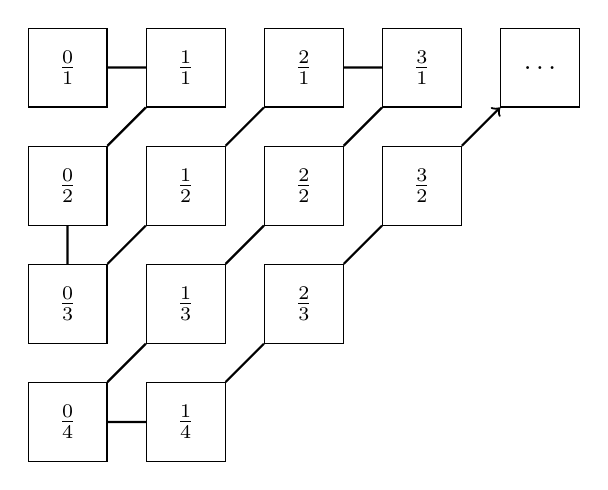
\begin{tikzpicture}[node distance=1.5cm, every node/.style={draw, minimum size=1cm, anchor=center}]
  \node (r01) {$\frac{0}{1}$};
  \node (r11) [right of=r01] {$\frac{1}{1}$};
  \node (r21) [right of=r11] {$\frac{2}{1}$};
  \node (r31) [right of=r21] {$\frac{3}{1}$};
  \node (r41) [right of=r31] {$\ldots$};
  \node (r02) [below of=r01] {$\frac{0}{2}$};
  \node (r12) [right of=r02] {$\frac{1}{2}$};
  \node (r22) [right of=r12] {$\frac{2}{2}$};
  \node (r32) [right of=r22] {$\frac{3}{2}$};
  \node (r03) [below of=r02] {$\frac{0}{3}$};
  \node (r13) [right of=r03] {$\frac{1}{3}$};
  \node (r23) [right of=r13] {$\frac{2}{3}$};
  \node (r04) [below of=r03] {$\frac{0}{4}$};
  \node (r14) [below of=r13] {$\frac{1}{4}$};
  \draw[thick, ->] (r01) -- (r11) -- (r02) -- (r03) -- (r12) -- (r21) -- (r31) -- (r22) -- (r13) -- (r04) -- (r14) -- (r23) -- (r32) -- (r41);
\end{tikzpicture}
\end{center}

Because we can list all rational numbers in a sequence like \(r_0, r_1, r_2, r_3, \ldots\)), it is possible to find the
immediate predecessor and successor of a rational number \textbf{in this specific listing}. Of course, this listing is
not unique, so different listings may yield different immediate neighbors for the same rational number.

% =============================================================================
\section{Another example to show that we can't always trust our intuition in mathematics}
% =============================================================================

Based on our daily experiences, we might think that a function that behaves differently for rational and irrational
numbers would be discontinuous at the point where the behavior changes. However, this is not always the case, and we can
construct a function that is continuous at that point despite having different definitions for rational and irrational
numbers.

Consider the following function:

\[
f(x) =
\begin{cases}
  x & \text{if } x \in \mathbb{R} \setminus \mathbb{Q} \text{ (irrational numbers)} \\
  0 & \text{if } x \in \mathbb{Q}
\end{cases}
\]

We can prove that $f(x)$ is continuous at \(x = 0\) as follows.

First of all, we know that \(f(0) = 0\) since 0 is a rational number. Therefore, we have:

\[|(f(x) - f(0)| = |f(x) - 0| = |f(x)| \leqslant |x|\]

because for irrational numbers, \(f(x) = x\), and for rational numbers, \(f(x) = 0 \leqslant |x|\). In both cases, the
absolute value of \(f(x)\) is less than or equal to the absolute value of \(x\).

Therefore, $\forall \epsilon > 0$, we can choose $\delta = \epsilon$ such that if $0 < |x - 0| = |x| < \delta$, then
$|f(x) - f(0)| = |f(x)| \leqslant |x| < \delta = \epsilon$. Therefore, by the definition of continuity, we have shown
that $f(x)$ is continuous at \(x = 0\).

By intuition, one might think that the continuity at \(x = 0\) means the left and right ``immediate neighbors'' of 0,
denoted by $x_l$ and $x_r$, must be both rational numbers too, such that $f(x_l) = f(x_r) = f(x) = 0$ in order to make
the changes from both the left and the right sides ``smooth'' without any abruptive ``jumps''. However, we can't find
such ``immediate neighbors'' because there are infinitely many rational and irrational numbers between any two real
numbers, so there is no immediate neighbor in the usual sense. This is sort of counter-intuitive: as $x$ approaches 0,
$x$ changes in between rational and irrational numbers, so $f(x)$ changes in between 0 and an irrational number. Because
$x > 0$, $f(x) > 0$ when $x \in \mathbb{R} \setminus \mathbb{Q}$, the function values approach 0 but with smaller and
smaller ``abruptive jumps'', but eventually, and \textbf{magically}, the function values reach 0 at $x = 0$ without any
jump. This is a very interesting example that shows how our intuition can be challenged when dealing with infinite
processes and the density of rational and irrational numbers on the real number line.

% =============================================================================
\section{Continuity}
% =============================================================================

In mathematics, ``continuity'' is defined as ``given a certain distance $\epsilon > 0$, I can \textbf{always} get
\textbf{closer} to the target point''. Eventually, you will find that the only case that you can make me unable to give
a closer distance is to make $epsilon = 0$. But when there is no distance between the two points, that means they are
``connected'' together, which is the essence of continuity.

% =============================================================================
\section{Binomial Theorem}
% =============================================================================

The Binomial Theorem describes the algebraic expansion of powers of a binomial. According to the theorem, it is possible
to expand the expression \((x + y)^n\) into a sum involving terms of the form \(ax^by^c\), where the coefficients \(a\)
are known as \textbf{binomial coefficients}. The theorem is stated as follows:

\[(x + y)^n = \sum_{k=0}^{n} \binom{n}{k} x^{n-k} y^k\]

where \(\binom{n}{k} = \frac{n!}{k!(n-k)!}\) is the binomial coefficient, representing the number of ways to choose \(k\)
elements from a set of \(n\) elements.

\textbf{Proof}: We can prove the Binomial Theorem using mathematical induction.

\textbf{Base Case} (\(n = 0\)): When \(n = 0\), we have:

\[(x + y)^0 = 1\]

The right-hand side of the theorem also gives:

\[\sum_{k=0}^{0} \binom{0}{k} x^{0-k} y^k = \binom{0}{0} x^0 y^0 = \frac{0!}{0!(0-0)!} x^0 y^0 = 1\]

Thus, the base case holds.

\textbf{Inductive Step}: Assume the theorem holds for some integer \(n = m\), i.e.:

\[(x + y)^m = \sum_{k=0}^{m} \binom{m}{k} x^{m-k} y^k\]

We need to show that it holds for \(n = m + 1\):

\[(x + y)^{m+1} = (x + y)(x + y)^m\]

Using the inductive hypothesis, we can substitute:

\[(x + y)^{m+1} = (x + y) \sum_{k=0}^{m} \binom{m}{k} x^{m-k} y^k\]

Expanding this, we get:

\[(x + y)^{m+1} = \sum_{k=0}^{m} \binom{m}{k} x^{m-k+1} y^k + \sum_{k=0}^{m} \binom{m}{k} x^{m-k} y^{k+1}\]

We can reindex the second sum by letting \(j = k + 1\):

\[(x + y)^{m+1} = \sum_{k=0}^{m} \binom{m}{k} x^{m-k+1} y^k + \sum_{j=1}^{m+1} \binom{m}{j-1} x^{m-(j-1)} y^j\]

In the first sum, we can take the term when \(k = 0\) separately, so we have:

\begin{align*}
  \sum_{k=0}^{m} \binom{m}{k} x^{m-k+1} y^k & = \binom{m}{0} x^{m+1} y^0 + \sum_{k=1}^{m} \binom{m}{k} x^{m-k+1} y^k \\
                                            & = \binom{m}{0} x^{m+1} + \sum_{k=1}^{m} \binom{m}{k} x^{m-k+1} y^k
\end{align*}

Likewise, in the second sum, we can take the term when \(j = m + 1\) separately, so we have:

\begin{align*}
  \sum_{j=1}^{m+1} \binom{m}{j-1} x^{m-(j-1)} y^j & = \sum_{j=1}^{m} \binom{m}{j-1} x^{m-(j-1)} y^j + \binom{m}{m} x^0 y^{m+1} \\
                                                  & = \sum_{k=1}^{m} \binom{m}{k-1} x^{m-k+1} y^k + \binom{m}{m} y^{m+1}
\end{align*}

Putting the two sums together and combining them, we have:

\begin{align*}
  (x + y)^{m+1} & = \binom{m}{0} x^{m+1} + \sum_{k=1}^{m} \binom{m}{k} x^{m-k+1} y^k + \\
                & + \sum_{k=1}^{m} \binom{m}{k-1} x^{m-k+1} y^k + \binom{m}{m} y^{m+1} \\
                & = \binom{m}{0} x^{m+1} + \sum_{k=1}^{m} \left(\binom{m}{k} + \binom{m}{k-1}\right) x^{m-k+1} y^k + \binom{m}{m} y^{m+1}
\end{align*}

Using the property of binomial coefficients:

\[\binom{m}{k} + \binom{m}{k-1} = \binom{m+1}{k}\]

and

\[\binom{m}{0} = \binom{m+1}{0}\]

and

\[\binom{m}{m} = \binom{m+1}{m+1}\]

we can rewrite the expression as:

\begin{align*}
  (x + y)^{m+1} & = \binom{m+1}{0} x^{m+1} + \sum_{k=1}^{m} \binom{m+1}{k} x^{m-k+1} y^k + \binom{m+1}{m+1} y^{m+1} \\
                & = \sum_{k=0}^{m+1} \binom{m+1}{k} x^{(m+1)-k} y^k
\end{align*}

Thus, the inductive step holds. By the principle of mathematical induction, the Binomial Theorem is proven for all
non-negative integers \(n\).

% ******************************
\subsection{Prove $\binom{m}{k} + \binom{m}{k-1} = \binom{m+1}{k}$}
% ******************************

\textbf{Proof}:
\begin{equation*}
  \begin{split}
    \binom{m}{k} + \binom{m}{k-1}
    & = \frac{m!}{k!(m-k)!} + \frac{m!}{(k-1)!(m-(k-1))!} \\
    & = \frac{m! (m - k + 1)}{k!(m-k+1)!} + \frac{m! k}{k!(m-k+1)!} \\
    & = \frac{m! (m + 1)}{k!(m-k+1)!} \\
    & = \frac{(m + 1)!}{k!((m + 1) - k)!} \\
    & = \binom{m+1}{k}
  \end{split}
\end{equation*}

% ******************************
\subsection{Prove $\binom{m}{0} = \binom{m+1}{0}$}
% ******************************

\textbf{Proof}:
\begin{equation*}
  \begin{split}
    \binom{m}{0} & = \frac{m!}{0!(m-0)!} = \frac{m!}{0! m!} = 1 \\
    \binom{m+1}{0} & = \frac{(m+1)!}{0!(m+1-0)!} = \frac{(m+1)!}{0! (m+1)!} = 1
  \end{split}
\end{equation*}

Thus

\[\binom{m}{0} = \binom{m+1}{0}\]

% ******************************
\subsection{Prove $\binom{m}{m} = \binom{m+1}{m+1}$}
% ******************************

\textbf{Proof}:
\begin{equation*}
  \begin{split}
    \binom{m}{m} & = \frac{m!}{m!(m-m)!} = \frac{m!}{m! 0!} = 1 \\
    \binom{m+1}{m+1} & = \frac{(m+1)!}{(m+1)!(0)!} = \frac{(m+1)!}{(m+1)! 0!} = 1
  \end{split}
\end{equation*}

Thus

\[\binom{m}{m} = \binom{m+1}{m+1}\]

\end{document}
